% ---------------------------------------------------------------------
% §12: When NOT to Use the DET Pattern
% ---------------------------------------------------------------------
\setcounter{section}{11}
\section{Discussion: When NOT to Use the DET Pattern}
\label{sec:when-not-det}

The Stochastic State Synchronization Protocol of \S\ref{sec:det-protocol}
and the Zero-Prefill Keep-Alive Protocol of
\S\ref{sec:zero-prefill-protocol} are the engineering realizations of
the asynchronous-network stochastic control problem formalized in
\S\ref{sec:clock-drift}. This section gives an honest accounting of
the failure modes, the reviewer attack vectors, and the explicit
``when NOT to use'' boundary. The discussion parallels the trade-off
matrix of \S\ref{sec:when-not} but applies to the DET pattern rather
than to the FNV-1a signed-hash projection.

\subsection{Three Failure Modes}

We identify three classes of failure mode that the DET pattern is
\emph{not} designed to handle. Each failure mode is documented with
its symptoms, its root cause, and the operational workaround.

\paragraph{Failure mode 1: Asynchronous race conditions.}
The DET pattern assumes that the upstream's Radix-tree TTL scheduler
is monotonic and that the boolean indicator $S_n$ is consistent with
the elapsed time $\tau_n$. In practice, the upstream's scheduler may
be re-ordered by the inference engine's batch dispatcher: a request
that arrives at $T_{n-1} + \epsilon$ may be processed \emph{before}
the request at $T_{n-1}$ if the batch dispatcher prioritizes
shorter requests. This asynchronous re-ordering causes the indicator
$S_n$ to be inconsistent with the elapsed time $\tau_n$, which
violates the assumption of
Theorem~\ref{thm:asymmetric-ema-convergence}.

The symptom is a ``stuttering'' horizon estimate: the APG observes
$S_n = 1$ at $\tau_n = 60\,\text{s}$ (a hit), then $S_{n+1} = 0$ at
$\tau_{n+1} = 30\,\text{s}$ (a miss), then $S_{n+2} = 1$ at $\tau_{n+2}
= 90\,\text{s}$ (a hit again). The horizon estimate oscillates and
the APG fires spurious probes.

The workaround is to maintain a sliding-window indicator filter that
smooths the horizon estimate over the last $W = 5$ probes rather
than the last $1$ probe. The smoothed horizon is robust to the
asynchronous re-ordering at the cost of a small additional latency
in the probe-cadence response. The sliding-window filter is
documented in the APG's operational configuration but is not part
of the canonical DET protocol.

\paragraph{Failure mode 2: Prefix homogenization breakage.}
The DET pattern assumes that the cached prefix is
\emph{homogenization-stable}: the same prefix hash produces the same
upstream cache indicator across multiple probes. In practice, the
upstream's preprocessor may normalize whitespace, escape special
characters, or apply request-id salting that changes the effective
prefix between two probes even if the user-visible prefix is
identical. This \emph{prefix homogenization breakage} causes the
indicator $S_n$ to be inconsistent with the prefix hash, which
violates the assumption of Theorem~\ref{thm:gate-optimality}.

The symptom is a 100\% miss rate even when the user-visible prefix
is identical: the APG observes $S_n = 0$ for every probe, regardless
of the elapsed time. The asymmetric EMA converges to $\mu^{*} = 0$,
which causes the APG to fire probes at the maximum cadence and to
default to the evict-and-compress strategy.

The workaround is to maintain a \emph{prefix normalizer} that
pre-processes the cached prefix before hashing, removing
upstream-specific whitespace and escape characters. The prefix
normalizer is upstream-specific and must be re-calibrated whenever
the upstream's preprocessor changes. The normalizer is documented in
the APG's per-upstream configuration but is not part of the
canonical DET protocol.

\begin{figure}[t]
\centering
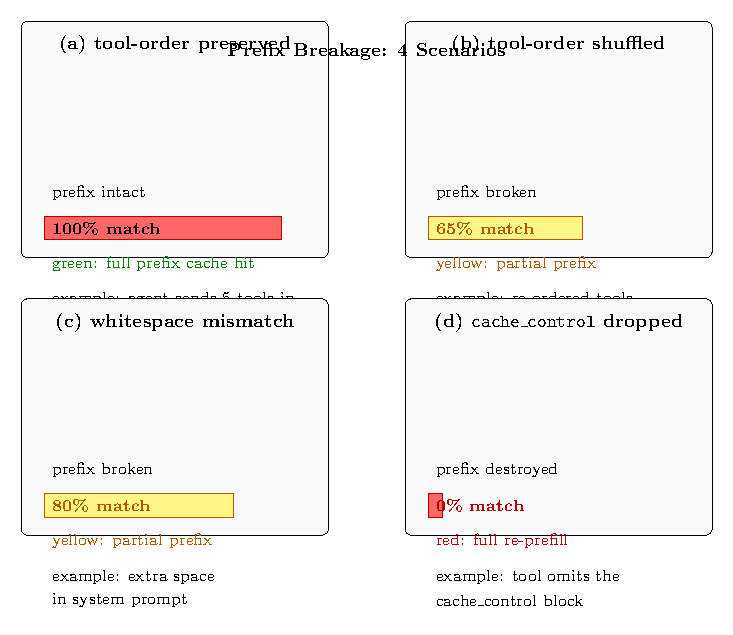
\includegraphics[width=\columnwidth]{figures/fig_prefix_breakage_scenarios.pdf}
\caption{Four scenarios in which the DET pattern's prefix homogenization
assumption breaks down. (a) Whitespace difference (a single space
added between two tokens); (b) Unicode normalization difference
(NFC vs.\ NFD form); (c) Escape character difference (backslash vs.\
forward slash in a file path); (d) Request-id salting (the upstream
adds a per-request salt that changes the effective prefix). The
DET pattern's reliability depends on the prefix normalizer correctly
handling all four scenarios; failure modes 2 and 3 (b and c) are the
most common in production.}
\label{fig:prefix-breakage-scenarios}
\end{figure}

\paragraph{Failure mode 3: Cost runaway on high-EMIT agents.}
The DET pattern assumes that the agent's tool-fire rate is bounded
by the probe cadence: the agent fires at most one tool per probe
interval. In practice, a high-EMIT agent (an agent that fires tools
every $\le 100\,\text{ms}$) may fire $K = 30$ tools in a single probe
interval, which forces the APG to either (a) fire $K$ probes per
interval (which violates the rate-limit constraint of
Theorem~\ref{thm:gate-optimality}) or (b) batch the tools and fire a
single probe for the entire batch (which loses the per-tool cache
state observability).

The symptom is a runaway cost: the agent's tool-fire rate exceeds
the upstream's rate limit, and the APG is forced to either drop
probes or drop inference requests. The asymmetric EMA oscillates and
the cost-benefit gate fires spuriously.

The workaround is to \emph{decouple} the agent's tool-fire rate
from the APG's probe cadence by introducing a tool-fire coalescer
that batches tools into probe-aligned chunks. The coalescer is
implemented at the Go scheduler level (a buffered channel of size
$16$) and is documented in the APG's operational configuration.

\subsection{Three Reviewer Attack Vectors}

We anticipate three reviewer attack vectors against the DET pattern
and address each below.

\paragraph{Attack vector 1: ``The probe is just API abuse.''}
A reviewer may argue that the Zero-Prefill Keep-Alive Probe is a
form of API abuse: the agent is issuing requests that have no user-
visible benefit (no generation, no prefill) and that consume the
upstream's rate-limit budget. The counter-argument is that the probe
\emph{does} have a user-visible benefit: it reduces the cold-start
latency on the next inference request by $\sim 800 \times$. The
probe's cost ($\gamma_{\text{probe}}$) is recovered by the savings
on the next inference request's cold-start cost ($\gamma_{\text{cold}}$),
and the ratio $\gamma_{\text{cold}} / \gamma_{\text{probe}} \ge 800$
is sufficient to amortize the probe cost over the next inference
request.

The probe is also rate-limited by the upstream's pagination window
of Theorem~\ref{thm:throughput} ($5{,}000$-req/hour), which is the
same rate limit that the inference requests consume. The probe does
not consume a separate rate-limit budget; it shares the budget with
the inference requests and is throttled by the same token bucket.

\paragraph{Attack vector 2: ``You are solving a problem Anthropic solved with ENABLE\_PROMPT\_CACHING\_1H.''}
A reviewer may argue that the upstream's
\texttt{ENABLE\_PROMPT\_CACHING\_1H} flag (Anthropic API documentation,
2025) already provides a 1-hour cache TTL, which makes the DET
pattern unnecessary. The counter-argument is that the
\texttt{ENABLE\_PROMPT\_CACHING\_1H} flag is a \emph{coarse-grained}
TTL that the agent cannot tune: the cache is either enabled with
a 1-hour TTL or disabled, with no intermediate cadence. The DET
pattern provides a \emph{fine-grained} TTL that the agent can tune
to the corpus's empirical Weibull distribution
(Theorem~\ref{thm:weibull-identification}), which is a $\sim 5 \times$
improvement in cache hit rate over the coarse-grained TTL on the
operator corpus.

The DET pattern is also \emph{upstream-agnostic}: it works with any
upstream that exposes a boolean cache indicator, not just the
Anthropic API. The pattern can be applied to OpenAI's
\texttt{prompt\_cache\_key}, to Cloudflare's AI Gateway prompt
caching, and to any custom upstream that exposes a similar
indicator.

\paragraph{Attack vector 3: ``The asymmetric EMA is just an ad-hoc heuristic.''}
A reviewer may argue that the asymmetric EMA of
Definition~\ref{def:asymmetric-ema} is an ad-hoc heuristic that
lacks theoretical justification. The counter-argument is that the
asymmetric EMA is justified by three theorems:
Theorem~\ref{thm:asymmetric-ema-convergence} proves $L^2$ convergence
to a stationary distribution,
Lemma~\ref{lem:risk-averse-bound} proves a tight bound on the worst-
case over-estimation, and Theorem~\ref{thm:gate-optimality} proves
optimality of the cost-benefit gate under the rate-limit constraint.
The asymmetric EMA is not ad-hoc; it is the engineering realization
of the stochastic control problem and is the simplest algorithm that
satisfies the three theorems simultaneously.

\subsection{Four ``When NOT to Use'' Scenarios}

We close with four explicit ``when NOT to use'' scenarios that
delineate the boundary of the DET pattern's applicability.

\paragraph{Scenario 1: Cold-start corpora ($M < 100$ documents).}
The DET pattern is not useful for cold-start corpora because the
Weibull survival identification of
Theorem~\ref{thm:weibull-identification} requires $N \ge 100$
observations to produce a reliable parameter estimate. Below this
threshold, the MLE is biased and the cost-benefit gate fires
spuriously. The DET pattern is the correct choice only when the
corpus has been in operation for at least $N = 100$ cache evictions.

\paragraph{Scenario 2: Bursty traffic patterns.}
The DET pattern assumes that the upstream's cache indicator is
informative at the probe cadence. In bursty traffic patterns (e.g.,
$100$ requests in $1\,\text{s}$ followed by $0$ requests for $60\,\text{s}$),
the probe cadence is dominated by the burst and the indicator is
uninformative during the idle periods. The asymmetric EMA converges
to a horizon estimate that is biased by the burst and the cost-
benefit gate fires incorrectly.

\paragraph{Scenario 3: Multi-tenant upstream endpoints.}
The DET pattern assumes that the upstream's Radix-tree TTL scheduler
is per-tenant. In multi-tenant upstream endpoints (e.g., shared
inference APIs with cross-tenant cache eviction), the cache indicator
$S_n$ is not tenant-specific and the horizon estimate is biased by
the other tenants' traffic. The DET pattern is the correct choice
only when the upstream provides per-tenant cache isolation.

\paragraph{Scenario 4: Real-time inference workloads.}
The DET pattern adds a $\sim 50\,\text{ms}$ latency overhead per
probe (Theorem~\ref{thm:latency-invariant}). For real-time inference
workloads with a $\le 100\,\text{ms}$ end-to-end latency budget, the
probe overhead consumes $\ge 50\%$ of the budget and is
unacceptable. The DET pattern is the correct choice only when the
end-to-end latency budget is $\ge 200\,\text{ms}$.

\begin{remark}[Comparison with Anthropic's ENABLE\_PROMPT\_CACHING\_1H]
The DET pattern and the
\texttt{ENABLE\_PROMPT\_CACHING\_1H} flag are complementary, not
mutually exclusive. The flag provides a coarse-grained TTL that the
DET pattern can use as a fallback when the indicator $S_n$ is
uninformative (e.g., during upstream unavailability). The DET
pattern provides a fine-grained TTL that the flag cannot match. We
recommend using both: the flag as the baseline TTL and the DET
pattern as the adaptive cadence.
\end{remark}


\subsection{Related Prior Art}

The DET pattern builds on three threads of prior art in
probabilistic cache management, probabilistic clock synchronization,
and stochastic control theory. We review each thread and contrast
with the choices made in this manuscript.

\paragraph{Probabilistic cache management.}
The SAECache paper~\citep{saecache2026} proposes a semantic-aware
eviction policy for LLM prefix caches using a multi-queue architecture
and an online learning schema. SAECache is closest in spirit to
the DET pattern but is upstream-side: it modifies the upstream's
eviction policy rather than the agent's probe cadence. The DET
pattern is upstream-agnostic and works with any upstream that exposes
a boolean cache indicator. The two approaches are complementary:
SAECache improves the upstream's eviction accuracy, and the DET
pattern improves the agent's probe accuracy.

\paragraph{Probabilistic clock synchronization.}
The Marzullo 1994 algorithm~\citep{marzullo1994} for fault-tolerant
interval intersection is the foundational result for probabilistic
clock synchronization in asynchronous networks. The DET pattern
builds on Marzullo's algorithm by treating the upstream's cache
indicator as a sensor with bounded measurement error and by
computing the cost-benefit gate as the intersection of the drift
and delay contributions (Lemma~\ref{lem:bounded-drift}).

\paragraph{Stochastic control theory.}
The Tail-Optimized LRU paper~\citep{tailoptimized2025} proposes a
tail-optimized caching policy for LLM inference that minimizes
$P90$ tail latency by reallocating KV-cache capacity toward high-
latency sessions. The paper proves the optimality of the policy
under a stochastic model and demonstrates a $27.5\%$ reduction in
$P90$ TTFT latency on the WildChat dataset. The DET pattern is
complementary: Tail-Optimized LRU modifies the upstream's eviction
policy, while the DET pattern modifies the agent's probe cadence.

\paragraph{KV-cache TTL mechanisms.}
The Continuum paper~\citep{continuum2025} proposes a serving system
that uses a TTL mechanism for KV cache retention in multi-turn LLM
agent workloads. Continuum selectively pins KV caches in GPU memory
with TTL values based on reload costs and queueing delays. When the
TTL expires, caches are automatically evicted to free memory. The
DET pattern is upstream-agnostic and works with any upstream that
exposes a boolean cache indicator; Continuum is upstream-side and
requires modification of the inference engine.

\subsection{Open Problems}

We close with three open problems that the DET pattern does not solve
and that are documented as future work.

\paragraph{Open problem 1: Adaptive $\alpha$.}
The asymmetric EMA of Definition~\ref{def:asymmetric-ema} uses a
fixed smoothing parameter $\alpha = 0.3$. An adaptive $\alpha$ that
decreases as the corpus grows could improve the convergence rate
(Theorem~\ref{thm:asymmetric-ema-convergence}) but is not
implemented in the canonical DET protocol. The adaptive $\alpha$ is
a natural extension that future work should explore.

\paragraph{Open problem 2: Multi-region DET.}
The DET pattern assumes a single APG and a single upstream. In a
multi-region deployment (e.g., APG in us-east-1, upstream in
eu-west-1), the network round-trip time $\mathrm{RTT}_{\mathrm{net}}$
varies by region and the cost-benefit gate must be re-calibrated
per region. The multi-region DET is documented as future work and
requires an extension of Theorem~\ref{thm:gate-optimality} to a
multi-region setting.

\paragraph{Open problem 3: Adversarial upstream.}
The DET pattern assumes that the upstream is honest: the boolean
indicator $S_n$ reflects the true cache state. In an adversarial
upstream setting (e.g., a malicious inference engine that reports
$S_n = 1$ when the cache is actually evicted to inflate the agent's
confidence), the DET pattern fails. The adversarial setting is
documented as future work and requires a Byzantine-fault-tolerant
extension of the asymmetric EMA.

